\documentclass[preview]{standalone}
\usepackage{amsmath}
\usepackage{amssymb}
\usepackage{stellar}
\usepackage{definitions}
\usepackage{bettelini}
\usepackage{tikz}
\begin{document}
\id{diffeq-bernoulli}
\genpage
\section{Bernoulli equations}

\begin{snippetdefinition}{bernoulli-equation-definition}{Bernoulli equation}
    Let \(I\) be an open interval, \(p,q\in C(I)\), and
    \(\gamma\in\realnumbers\setminus\{0,1\}\).
    A \emph{Bernoulli equation} is
    \[
        y'=p(x)y+q(x)y^\gamma.
    \]
    For arbitrary real \(\gamma\) the natural real domain is \(I\times(0,+\infty)\).
    Other values of \(y\) may be admitted when the power is defined, for instance
    all real \(y\) for a positive integer exponent.
\end{snippetdefinition}

\begin{snippettheorem}{bernoulli-equation-sol}{Reduction to a linear equation}
    Let \(p,q\in C(I)\), \(\gamma\neq0,1\), and let \(y>0\) on an open interval
    \(I\). Then \(y\) solves \(y'=py+qy^\gamma\)
    \ifandonlyif \(z=y^{1-\gamma}>0\) solves
    \[
        z'=(1-\gamma)pz+(1-\gamma)q.
    \]
    The inverse substitution is \(y=z^{1/(1-\gamma)}\), and
    \(y(x_0)=y_0>0\) becomes \(z(x_0)=y_0^{1-\gamma}\).
    The same reduction holds on other nonzero branches where the power
    substitution is real, differentiable and invertible.
\end{snippettheorem}

\begin{snippetproof}{bernoulli-equation-sol-proof}{bernoulli-equation-sol}{Reduction to a linear equation}
    Divide the equation by \(y^\gamma\):
    \[
        y^{-\gamma}y'=p y^{1-\gamma}+q.
    \]
    Since \(z'=(1-\gamma)y^{-\gamma}y'\), multiplication by \(1-\gamma\)
    yields the linear equation. Differentiating the inverse substitution
    proves the converse on the specified branch.
    In the notation \(y'+ay+by^\gamma=0\), the equation becomes
    \[
        z'+(1-\gamma)az+(1-\gamma)b=0.
    \]
\end{snippetproof}

\begin{snippetproposition}{diffeq-bernoulli-zero-solution}{The zero solution}
    Let \(p,q\in C(I)\) and \(\gamma>0\), \(\gamma\neq1\).
    If the real domain of \(y'=py+qy^\gamma\) includes \(y=0\),
    then \(y\equiv0\) is a solution. It is not represented by a substitution
    that requires \(y\neq0\).
\end{snippetproposition}

\begin{snippetnote}{diffeq-bernoulli-branches}{Positivity and uniqueness}
    For \(y_0>0\), continuity of \(p,q\) gives local existence and uniqueness
    on \(I\times(0,+\infty)\), because
    \(\partial_y(py+qy^\gamma)=p+\gamma qy^{\gamma-1}\) is continuous there.
    The transformed solution is usable only while the chosen branch remains valid.
    When \(0<\gamma<1\), the derivative of \(y^\gamma\) is singular at zero;
    uniqueness at zero cannot be concluded from this theorem.
\end{snippetnote}

\section{Examples}

\begin{snippetexample}{diffeq-bernoulli-quartic-example}{An integer exponent}
    Consider \(y'-y+xy^4=0\), \(y(0)=b\), with \(b\in\realnumbers\).
    The right-hand side \(y-xy^4\) is continuously differentiable on
    \(\realnumbers^2\). For \(b=0\), uniqueness gives \(y=0\).
    For \(b\neq0\), set \(z=y^{-3}\), using the real cube root for either sign.
    Then \(y=z^{-1/3}\), \(y'=-\tfrac13 z^{-4/3}z'\), and
    \[
        -\tfrac13 z^{-4/3}z'-z^{-1/3}+xz^{-4/3}=0
        \quad\Longleftrightarrow\quad z'+3z=3x.
    \]
    Since \(z(0)=b^{-3}\), the integrating-factor formula gives
    \[
        z(x)=e^{-3x}\left(b^{-3}+\integral[0][x][3te^{3t}][t]\right).
    \]
    Here
    \[
        \integral[0][x][3te^{3t}][t]
        =xe^{3x}-\frac13e^{3x}+\frac13,
    \]
    so
    \[
        z(x)=x-\frac13+\left(b^{-3}+\frac13\right)e^{-3x},
        \qquad
        y(x)=\frac1{\sqrt[3]{x-\frac13+(b^{-3}+\frac13)e^{-3x}}}.
    \]
    The maximal interval is the component containing zero on which the
    radicand is nonzero.
\end{snippetexample}

\begin{snippetexample}{diffeq-bernoulli-square-root-example}{A fractional exponent}
    Consider
    \[
        y'+\frac2{x+1}y-\frac{\sqrt y}{x^2-1}=0,\qquad
        y(0)=b\geq0.
    \]
    For \(b=0\), \(y=0\) is a solution on \((-1,1)\).
    For \(b>0\), first work on \((-1,1)\times(0,+\infty)\), where the
    right-hand side is continuously differentiable.
    Set \(z=\sqrt y>0\). Since \(y=z^2\), \(y'=2zz'\), substitution gives
    \[
        2zz'+\frac2{x+1}z^2-\frac z{x^2-1}=0.
    \]
    Dividing by \(2z\) yields
    \[
        z'+\frac z{x+1}=\frac1{2(x^2-1)},\qquad
        ((x+1)z)'=\frac1{2(x-1)}.
    \]
    Integrating from zero and using \(z(0)=\sqrt b\), we obtain
    \[
        (x+1)z(x)=\sqrt b+\frac12\ln(1-x),\qquad
        y(x)=\left(\frac{\sqrt b+\frac12\ln(1-x)}{x+1}\right)^2.
    \]
    This formula solves the original equation only where the numerator is positive,
    because the substitution requires \(z=\sqrt y\), not \(z=-\sqrt y\).
    It vanishes at
    \[
        x_1=1-e^{-2\sqrt b}.
    \]
    Thus the positive branch through \((0,b)\) has domain \((-1,x_1)\).
    The original sketch below illustrates its approach to zero; its axes are schematic.
\begin{center}
        \begin{tikzpicture}[scale=0.9]
            \draw[->] (-2.2,0) -- (3,0) node[right] {\(x\)};
            \draw[->] (0,-0.3) -- (0,2.5) node[above] {\(y\)};
            \draw[dashed] (-1,-0.2) -- (-1,2.3) node[above] {\(-1\)};
            \draw[dashed] (1.8,-0.2) -- (1.8,2.3) node[above] {\(x_1\)};
            \draw[domain=-0.9:1.75,samples=120] plot (\x,{0.65*(\x-1.8)^2});
            \fill (1.8,0) circle (1.3pt);
        \end{tikzpicture}
    \end{center}
\end{snippetexample}

\begin{snippetexample}{diffeq-bernoulli-gluing-example}{Nonunique continuation from zero}
    For
    \[
        y'+\frac2{x+1}y-\frac{\sqrt y}{x^2-1}=0
        \quad\text{on }(-1,1),
    \]
    fix \(c\in(-1,1)\). The \function
    \[
        y_c(x)=
        \begin{cases}
        \displaystyle\left(\frac{\ln((1-x)/(1-c))}{2(x+1)}\right)^2,
            &-1<x<c,\\[4pt]
        0,&c\leq x<1
        \end{cases}
    \]
    is continuously differentiable at \(c\): the positive branch and its derivative
    both tend to zero there. It therefore solves the equation on \((-1,1)\).
    It and \(y\equiv0\) are distinct solutions of the initial value problem \(y(c)=0\).
    More generally \(y_d\), for any \(d\leq c\) in \((-1,1)\), has \(y_d(c)=0\).
    For \(b>0\) in the preceding initial value problem, joining at
    \(c=x_1=1-e^{-2\sqrt b}\) extends its positive branch by zero.
    On \((-1,1)\), the right-hand side is strictly negative when \(y>0\).
    Thus a positive branch can arrive at zero from the left, but cannot depart
    from zero to the right.
\end{snippetexample}

\begin{snippet}{diffeq-bernoulli-original-gluing-sketches}
    The original four sketches are retained below as schematic illustrations
    of zero branches and possible junction shapes, not as four solutions of
    the displayed Bernoulli equation. For that equation on \((-1,1)\),
    only the zero graph and the decreasing-positive-then-zero shape are admissible.
    In particular, squaring a transformed solution after its sign changes
    does not produce a solution of the original equation.
\begin{center}
        \begin{tikzpicture}[scale=0.8]
            \draw[->] (-2,0) -- (2,0) node[right] {\(x\)};
            \draw[->] (0,-0.2) -- (0,1.8) node[above] {\(y\)};
            \draw[very thick] (-1.8,0) -- (1.8,0);
        \end{tikzpicture}
        \qquad
        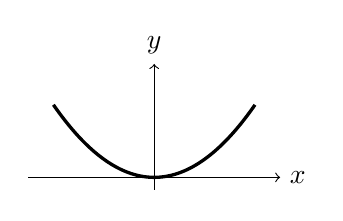
\begin{tikzpicture}[scale=0.8]
            \draw[->] (-2,0) -- (2,0) node[right] {\(x\)};
            \draw[->] (0,-0.2) -- (0,1.8) node[above] {\(y\)};
            \draw[domain=-1.6:1.6,samples=100,very thick] plot (\x,{0.45*\x*\x});
        \end{tikzpicture}
        \qquad
        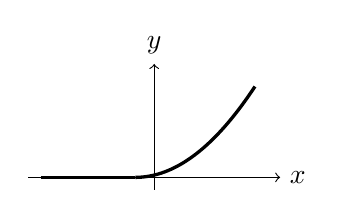
\begin{tikzpicture}[scale=0.8]
            \draw[->] (-2,0) -- (2,0) node[right] {\(x\)};
            \draw[->] (0,-0.2) -- (0,1.8) node[above] {\(y\)};
            \draw[very thick] (-1.8,0) -- (-0.3,0);
            \draw[domain=-0.3:1.6,samples=100,very thick] plot (\x,{0.4*(\x+0.3)^2});
        \end{tikzpicture}
        \qquad
        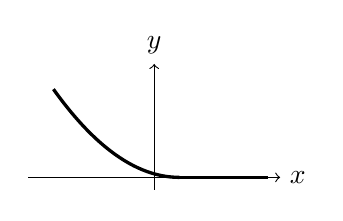
\begin{tikzpicture}[scale=0.8]
            \draw[->] (-2,0) -- (2,0) node[right] {\(x\)};
            \draw[->] (0,-0.2) -- (0,1.8) node[above] {\(y\)};
            \draw[domain=-1.6:0.4,samples=100,very thick] plot (\x,{0.35*(\x-0.4)^2});
            \draw[very thick] (0.4,0) -- (1.8,0);
        \end{tikzpicture}
    \end{center}
\end{snippet}

\end{document}
